\clearpage
\subsection{Interacting with Files} % (fold)
\label{sub:interacting_with_files}

Programming languages offer a number of functions and procedures that are used to interact with files. These will allow you to save data to a file, and load data back from the file.

\begin{figure}[h]
   \centering
   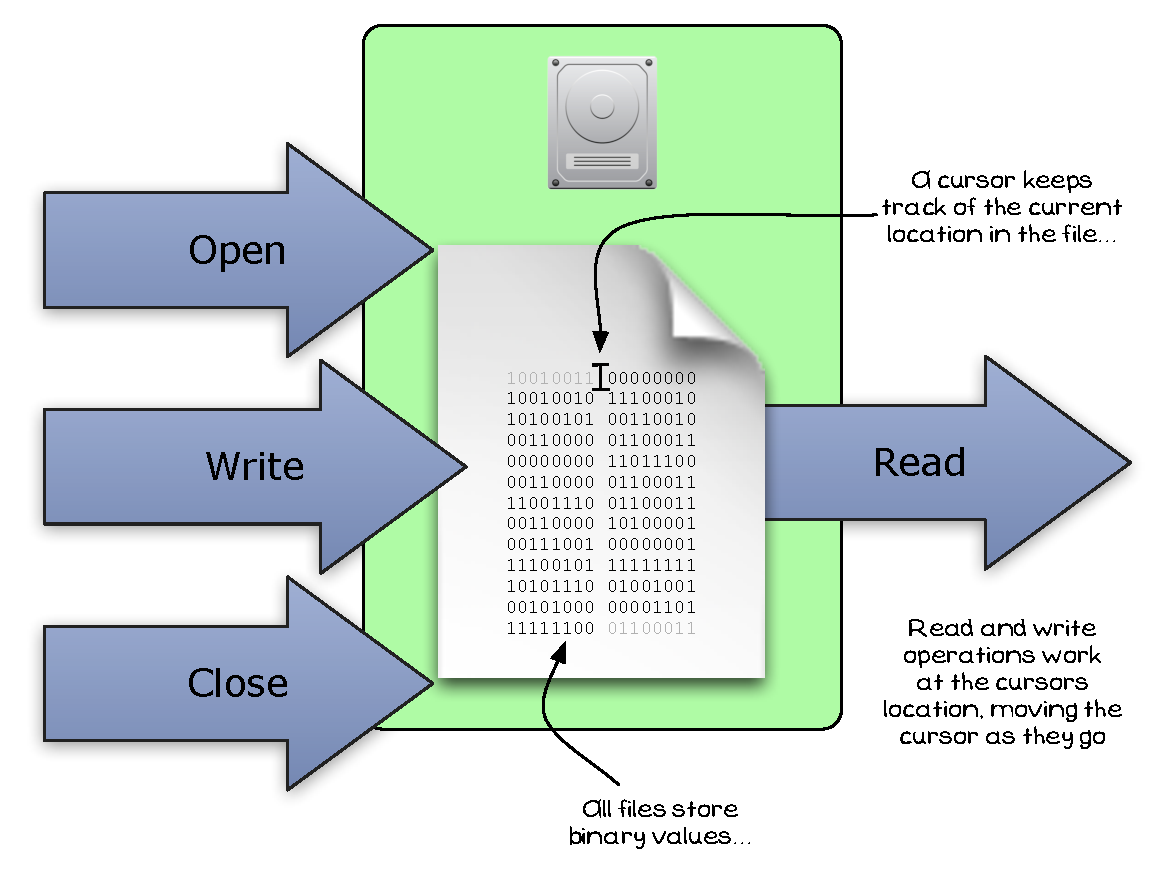
\includegraphics[width=\textwidth]{./topics/file-io/diagrams/FileOps} 
   \caption{File operations include the ability to open, read, write, and close files}
   \label{fig:file-ops}
\end{figure}

\mynote{
\begin{itemize}
  \item Programming languages will provide functions and procedures to:
  \begin{itemize}
    \item \textbf{Open} a file so you can interact with its contents.
    \item \textbf{Read} data from a file that has been opened to be read.
    \item \textbf{Write} data to a file that has been opened to be written to.
    \item \textbf{Close} a file that is currently open.
  \end{itemize}
  \item Languages will also provide built in file types that are used with these functions and procedures.
  \item When you open a file you indicate if you want read and/or write access to its contents.
  \item Opening a file gives you access to a cursor that you can use to read data from the file, or write data to the file.
  \item Standard usage will be to open the file, read/write data to the file, and then close the file.
\end{itemize}
}


% subsection interacting_with_files (end)